\documentclass{beamer}

\mode<presentation>{
	%\usetheme{CambridgeUS}
	%\usecolortheme{seahorse}
	\usetheme{Boadilla}
	\usecolortheme{beaver}
	\setbeamertemplate{navigation symbols}{}
}

\usepackage{graphicx}
\usepackage{booktabs}
\usepackage{algpseudocode}
\usepackage{hyperref}
\usepackage{tikz}
\usepackage[utf8]{inputenc}
\usepackage{listings}
\usepackage[export]{adjustbox}
\usepackage{aeguill}

%\setbeamertemplate{title page}[default][rounded=false]

\setbeamertemplate{title page}
{
%\vbox{}
\begingroup
\centering
\begin{beamercolorbox}[sep=8pt,center]{institute}
\usebeamerfont{institute}\insertinstitute
\end{beamercolorbox}
\vskip1em%
\begin{beamercolorbox}[sep=8pt,center]{title}
\usebeamerfont{title}\inserttitle\par%
\ifx\insertsubtitle\@empty%
\else%
\vskip0.25em%
{\usebeamerfont{subtitle}\usebeamercolor[fg]{subtitle}\insertsubtitle\par}%
\fi%
\end{beamercolorbox}%
\vfill
\begin{beamercolorbox}[sep=8pt,center]{author}
\usebeamerfont{author}\insertauthor
\end{beamercolorbox}
\vskip1em\par
\begin{beamercolorbox}[sep=8pt,center]{date}
\usebeamerfont{date}\insertdate
\end{beamercolorbox}
\endgroup
}

\setbeamertemplate{blocks}[default]
\setbeamercolor{structure}{fg=darkred}
%\setbeamercolor{block title}{bg=darkred,fg=white}
%\setbeamercolor{block body}{bg=darkgray!20!white}
\setbeamercolor{block title}{bg=darkgray!30!white}
\setbeamertemplate{enumerate items}[default]

\setbeamertemplate{part page}{
\begin{beamercolorbox}[sep=8pt,center,wd=\textwidth]{part title}
\usebeamerfont{part title}\insertpart\par
\end{beamercolorbox}
\vfill
\tableofcontents
}

%\setbeamertemplate{frametitle continuation}{(\insertcontinuationcount)}

\setbeamertemplate{headline}{\leavevmode\hbox{\begin{beamercolorbox}[wd=.5\paperwidth,ht=2.65ex,dp=1.5ex,center]{section in head/foot}\usebeamerfont{section in head/foot}\insertsectionhead\hspace*{2ex}
\end{beamercolorbox}\begin{beamercolorbox}[wd=.5\paperwidth,ht=2.65ex,dp=1.5ex,center]{subsection in head/foot}\usebeamerfont{subsection in head/foot}\hspace*{2ex}\insertsubsectionhead\end{beamercolorbox}}\vskip0pt}

\setbeamertemplate{background}{\tikz[overlay,remember picture]\node[opacity=0.08]at (current page.south east){
\includegraphics[width=10cm]{figures/unibo_logo.jpg}};}

\newcommand{\tcc}[1]{\textcolor{darkred}{#1}}

\newcommand{\codeA}[1]{\texttt{#1}}
\newcommand{\codeB}[1]{\texttt{\textcolor{darkred}{#1}}}

\newcommand{\link}[1]{{\footnotesize » \url{#1}}}
\newcommand{\bothquote}[1]{``#1''}

\definecolor{mygreen}{rgb}{0,0.6,0}
\definecolor{mygray}{rgb}{0.5,0.5,0.5}
\definecolor{mymauve}{rgb}{0.58,0,0.82}
\definecolor{maroon}{rgb}{0.5,0,0}
\definecolor{darkgreen}{rgb}{0,0.5,0}

\lstset{
language=Java,
basicstyle=\scriptsize\ttfamily,
keywordstyle=\scriptsize\color{blue}\ttfamily,
commentstyle=\scriptsize\color{mygreen}\ttfamily,
breakatwhitespace=false,
breaklines=true,
 numbers=left,
  numberstyle=\color{mymauve},
  stringstyle=\color{mymauve},
  showstringspaces=false,
  numbers=none
}

\lstdefinelanguage{XML}
{
  basicstyle=\scriptsize\ttfamily,
  morestring=[s]{"}{"},
  morecomment=[s]{?}{?},
  morecomment=[s]{!--}{--},
  commentstyle=\color{darkgreen},
  moredelim=[s][\color{black}]{>}{<},
  moredelim=[s][\color{red}]{\ }{=},
  stringstyle=\color{blue},
  identifierstyle=\color{maroon},
  numbers=none
}

\makeatother

\AtBeginSection[]
{
  \begin{frame}
    \frametitle{Outline}
    \tableofcontents[currentsection]
  \end{frame}
}

%\AtBeginSubsection[]
%{
%  \begin{frame}
%    \frametitle{Outline}
%    \tableofcontents[currentsection,currentsubsection]
%  \end{frame}
%}

\institute[UNIBO]{\uppercase{Alma Mater Studiorum -- Università di Bologna}\\Dipartimento di Informatica -- Scienza e Ingegneria (DISI)\\C.d.S. in Ingegneria e Scienze Informatiche, Campus di Cesena}

\author[A. Marfoglia]{Alberto Marfoglia\\\scriptsize\texttt{alberto.marfoglia2@unibo.it}}


\title[Android -- 2B -- GUI]{Android Programming}
\subtitle{GUI, Resources and Shared Preferences}
\date[ver. 1.0 (20220505)]{Embedded Systems and Internet of Things\\A.A. 2021 -- 2022}

\begin{document}

  \begin{frame}
    \titlepage
  \end{frame}

  \newcommand\blfootnote[1]{%
  \begingroup
  \renewcommand\thefootnote{}\footnote{#1}%
  \addtocounter{footnote}{-1}%
  \endgroup
}

\begin{frame}{Thanks}
    \centering
    \begin{itemize}
      \item \large{Professor Angelo Croatti}
    \end{itemize}

    \blfootnote{\url{https://www.unibo.it/sitoweb/a.croatti/en}}
    \blfootnote{}
\end{frame}

  \begin{frame}
    \frametitle{Outline}
    \tableofcontents
  \end{frame}

\section{GUI Introduction}

  \begin{frame}{Approccio alle GUI in Android}
    \begin{itemize}\itemsep20pt
      \item Theoretically, a GUI for an Activity could be described and created
      programmatically (directly in the source code).
      \begin{itemize}
        \item Similarly to what can be done in java.
        \item First you create the instances of the graphic components (eg JButton),
        then they are associated with a layout (eg JPanel) and finally the layout is
        hooked to a window (eg JFrame).
      \end{itemize}
      \item In Android, however, we prefer to describe (and manage) graphical
      interfaces in another way. 
      \begin{itemize}
        \item By defining a GUI, and all its components, through resources.
        \item The description of the interfaces goes through writing XML files.
        \item From Android 5.0, you should follow the \tcc{Material Design}
        \textit{philosophy}.
      \end{itemize}
    \end{itemize}
  \end{frame}

\section{Android Resources}

  \begin{frame}{(Informal) Definition of Resource}
    \begin{itemize}\itemsep10pt
      \item Source code alone is not enough to write a good (well-designed)
      Android application. 
      \item \textbf{Resources are additional files for the application} 
      \begin{enumerate}
        \item written in XML language 
        \item with static content
        \item which can be referenced from the source code
        \item that allow you to describe a series of elements and
        characteristics of the application.
      \end{enumerate}
      
      \item You can create resources for: \tcc{layout} and graphic interfaces'
      components (\tcc{drawable}), \tcc{menus}, text for localization and
      dimensions (values), ...
    \end{itemize}
  \end{frame}

  \begin{frame}{Principle of Resource Indipendency}
    \begin{itemize}\itemsep10pt
      \item \textbf{Defining some elements as resources means keeping them
      independent of the application logic.}
    \begin{itemize}
      \item The resources can be chosen (through identifiers) and
      \bothquote{activated} at runtime.
    \end{itemize}
      \item ES1. \textit{If the GUI of an Activity is defined as a resource,
      multiple resources can be defined for the same GUI and the most
      appropriate one can therefore be chosen according to the screen size of
      the device on which the application will be executed.}
      \item ES2. \textit{Defining all messages and textual references of an
      application separately (through resources) allows you to facilitate the
      localization of the application (that is, the transition between one
      language and another).} 
    \end{itemize}
  \end{frame}

\subsection{The \texttt{R.java} file}
  \begin{frame}{The \texttt{R.java} file}
    \begin{itemize}\itemsep10pt
      \item The Android Development Kit automatically generates a file (R.java)
      with all references to the resources defined in the project. In this way,
      you can access resources with a logical name.
      \begin{itemize}
        \item Logical names are defined in the R file as a class hierarchy and
        are treated as static fields of type Integer.
      \end{itemize}
      \item Eg. When creating an activity, the reference to the resource that
      defines its layout must be passed to the \codeA{setContentView()} method.
      \begin{itemize}
        \item \codeB{setContentView(R.layout.myactivty\_layout)} 
        \item It means that there is the \codeA{myactivity\_layout} resource
        described in an XML file of the same name that defines a GUI layout.
      \end{itemize}
    \end{itemize}
  \end{frame}

\subsection{Resource Tree}

  \begin{frame}{Resource Tree di un'applicazione}

    \begin{columns}[c]
      \column{0.5\textwidth}
        \begin{itemize}\itemsep20pt
          \item In the project home directory there is a \codeB{res} directory for
          resources, organized in sub-directories.
          \item Other subdirectories can be added to contain specific resources.
        \end{itemize}
      \column{0.5\textwidth}
        \begin{figure}
          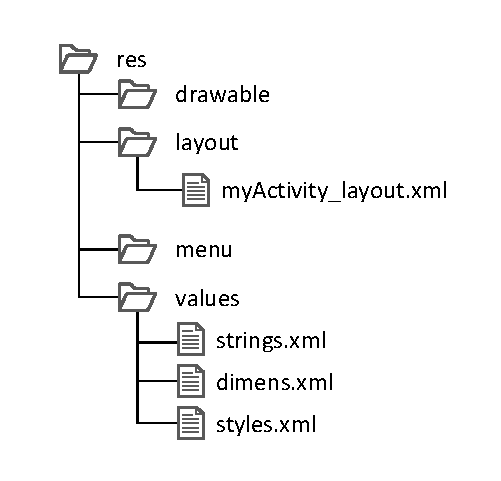
\includegraphics[width=1\linewidth]{figures/res-tree.pdf}
        \end{figure}
    \end{columns}
  \end{frame}

\section{Android GUI and Layout}
  \begin{frame}{Android User Interface}
    \begin{itemize}\itemsep20pt
      \item It represents everything the user can see and interact with directly.
      \begin{itemize}
        \item Generally a UI is associated with the Activity component. 
      \end{itemize}
      \item There are several predefined components to create and organize the
      application's layout.  
      \begin{itemize}
        \item One or more manageable events are associated with each component.
        \item One or more events are associated with each component, these can
        be managed through appropriate listeners.
        \item The names change, but the GUI management mechanism is (from a
        logical point of view) the same as that adopted in Swing in Java. 
      \end{itemize}
    \end{itemize}
  \end{frame}

\subsection{Component Hierarchy}
  \begin{frame}{Android UI -- Some Components}
    \begin{itemize}\itemsep10pt
      \item Layout Component 
      \begin{itemize}
        \item LinearLayout, RelativeLayout, FrameLayout, TableLayout,\dots
      \end{itemize}
      \item Input Component
      \begin{itemize}
        \item Button, TextField, CheckBox, RadioButton, Spinner, ToggleButton,\dots
      \end{itemize}
      \item Output Component
      \begin{itemize}
        \item TextView, ListView, GridView, ImageView, SurfaceView,\dots
      \end{itemize}
      \item \dots
    \end{itemize}
    \vfill
    \link{http://developer.android.com/guide/topics/ui/index.html}
  \end{frame}

  \begin{frame}[fragile]{GUI Definition -- Example}
    \begin{exampleblock}{\texttt{myactivity\_layout.xml}}
      \begin{lstlisting}[language=XML]  		        
      <?xml version="1.0" encoding="utf-8"?>
      <LinearLayout 
        xmlns:android="http://schemas.android.com/apk/res/android"
        android:layout_width="fill_parent" 
        android:layout_height="fill_parent"
        android:orientation="vertical">
        <TextView 
          android:id="@+id/mytextview"
          android:layout_width="wrap_content"
          android:layout_height="wrap_content"
          android:text="I am a TextView"/>
        <Button
          android:id="@+id/mybutton"
          android:layout_width="wrap_content"
          android:layout_height="wrap_content"
          android:text="I am a Button"/>
      </LinearLayout>
      \end{lstlisting}
    \end{exampleblock}
  \end{frame}

  \begin{frame}{Gui Definition -- Example (note) I}
    \begin{itemize}
      \item A resource called \codeA{myactivity\_layout} has been defined in the
      XML file of the same name.
      \begin{itemize} 
        \item It is automatically added to the R file by means of a static field
        of the same name in the \codeB{layout} subclass. 
      \end{itemize}
      \item The GUI is structured using a main linear layout of vertical type
      (whose components are aligned one below the other).
      \begin{itemize}
        \item Note. The outermost component of any layout must define the
        property that qualifies the file as an Android resource.
        \codeB{xmlns:android="http://schemas.android.com/apk/res/android"}
      \end{itemize}
      \item In the main linear layout, two components have been defined: a
      \codeA{textview} and a \codeA{button}.
    \end{itemize}
  \end{frame}
  \begin{frame}{Gui Definition -- Example (note) II}
    \begin{itemize}
      \item Some property values have been defined for both the layout and the
      components.
      \item Each component has been associated with a logical name which will be
      the one found in the R file. 
      \begin{itemize}
        \item Eg. As for the button, the \codeB{android:id} property has been
        assigned the value \codeB{@+id\/mybutton}
        \item This declares that you want to add a static field for subclass
        \codeB{id} named \codeB{mybutton} to the R file.
      \end{itemize}
    \end{itemize}
  \end{frame}

\subsection{Management of GUI elements}

  \begin{frame}[fragile,allowframebreaks]{Management of GUI elements}
    \begin{itemize}
      \item As seen in the description phase of the Activity component, the
      association of a GUI (a layout) must be done when creating the Activity.
      \begin{itemize}
        \item \textbf{Referring to the ID of the layout resource you want to
        associate}
      \end{itemize}
    \end{itemize}

    \begin{exampleblock}{Example -- Association of a GUI to an Activity}
      \begin{lstlisting}[language=Java]  		        
  @Override
  protected void onCreate(Bundle savedInstanceState){
    super.onCreate(savedInstanceState);
    setContentView(R.layout.activity_main);
      
    /* ... */
  }
      \end{lstlisting}
    \end{exampleblock}

    \begin{itemize}
      \item The reference to the elements of the GUI can be requested at any point
      of the activity through the \codeB{findViewById(int id)} method provided by
      the Activity class.
      \begin{itemize}
        \item Given the component identifier, it returns the relative generic
        type instance (\codeB{View}) that must be suitably converted to the
        specific type of the component.
      \end{itemize}
    \end{itemize}

    \begin{exampleblock}{Example -- Access to GUI elements}
      \begin{lstlisting}[language=Java]  		        
      Button btn = (Button) findViewById(R.id.mybutton);
      TextView txt = (TextView) findViewById(R.id.mytextview);
      \end{lstlisting}
    \end{exampleblock}

    \begin{itemize}
      \item Once the instance of the object associated with the graphic component
      has been obtained, it is possible to manage properties and events.
      \begin{itemize}
        \item For example, bind listeners to specific events or get/modify
        individual property values. 
      \end{itemize}
    \end{itemize}

    \begin{exampleblock}{Example -- Bind Listener to button click}
      \begin{lstlisting}[language=Java]  		        
Button btn = (Button) findViewById(R.id.mybutton);
btn.setOnClickListener(new OnClickListener(){	
  @Override
  public void onClick(View v) {
    //do something
  }	
});
      \end{lstlisting}
    \end{exampleblock}

    \begin{exampleblock}{Example -- Editing the TextView text}
      \begin{lstlisting}[language=Java]  		        
TextView txt = (TextView) findViewById(R.id.mytextview);
txt.setText("new text");
      \end{lstlisting}
    \end{exampleblock}
    \begin{small}
      \begin{itemize}
        \item Retrieves the component object instance which can then be handled
        similarly to what you would do in Java.
      \end{itemize}
    \end{small}
  \end{frame}

\subsection{Dialogs e Notifiche}

  \begin{frame}{Dialogs}
    \begin{itemize}\itemsep10pt
      \item A \tcc{Dialog} represents a popup generally used to communicate
      messages to the user, to propose a choice and/or request confirmation. 
      \item In Android there are several dialog types:
      \begin{itemize}
        \item \codeB{AlertDialog}, \codeB{DialogFragment},
        \codeB{ProgressDialog}, \dots
      \end{itemize}
      \item Each can be customized both in content and in layout (through a
      resource defined in XML).
    \end{itemize}
    \vfill
    \link{https://developer.android.com/guide/topics/ui/dialogs.html}
  \end{frame}

  \begin{frame}[fragile,allowframebreaks]{Alert Dialog}
      \begin{itemize}\itemsep10pt
        \item This is the simplest and most immediate alert available in Android
        (it is represented by the \codeB{AlertDialog} type)
        \item It can be created using the Builder pattern (\codeB{AlertDialog.Builder}) 
        \begin{itemize}
        \item The Builder must be instantiated with the reference to the activity
        that will have to display the dialog.
        \item The current activity can be returned from the \codeA{getActivity()}
        method of the Activity class. 
        \item The last method to call on the Builder is the \codeB{create()}
        method which returns the \codeA{AlertDialog} instance.
      \end{itemize}
    \end{itemize}

    \begin{exampleblock}{Example}
      \begin{lstlisting}[language=Java]  	
AlertDialog dialog = new AlertDialog.Builder(getActivity())
  .setTitle("File unsaved...")
  .setMessage("Do you want to save this file?")
  .setCancelable(false)
  .setPositiveButton("YES", new DialogInterface.OnClickListener() {
    public void onClick(DialogInterface dialog, int id) { 
      /* save file */ 
    }
  })
  .setNeutralButton("Undo", new DialogInterface.OnClickListener() {
    public void onClick(DialogInterface dialog, int id) {/*...*/}
  })
  .setNegativeButton("NO", new DialogInterface.OnClickListener() {
    public void onClick(DialogInterface dialog, int id) {/*...*/}
  })
  .create();
      \end{lstlisting}
    \end{exampleblock}
  \end{frame}

  \begin{frame}{Notifications}
    \begin{itemize}\itemsep10pt
      \item A notification is a message that can be proposed to the user by an
      application outside the application layout.
      \begin{itemize}
        \item It appears as an item in the notification bar of the device
      \end{itemize}
      \item In Android, there are two macro-types for notifications: 
      \begin{itemize}
        \item \tcc{Standard Notification}
        \item \tcc{Toast Notification}
      \end{itemize}
    \end{itemize}
    \vfill
    \link{developer.android.com/guide/topics/ui/notifiers/notifications.html}\\
    \link{developer.android.com/guide/topics/ui/notifiers/toasts.html}
  \end{frame}

  \begin{frame}[fragile,allowframebreaks]{Traditional Notifications}
    \begin{itemize}\itemsep10pt
      \item Also for notifications, the creation mechanism makes use of the
      pattern builder.
      \item Notification events are handled through \codeA{Intent}.
      \begin{itemize}
        \item In particular, through a specialization of the \codeB{Intent} class
        called \codeB{PendingIntent}.
      \end{itemize}
        \item Notifications can be viewed using the \codeB{NotificationManager}
        instance.
      \begin{itemize}
        \item Instance on which the \codeB{notify(int id, Notification n)} method
        can be called to send the notification.
        \item The Notification Manager can be obtained through the
        \codeB{getSystemService()} API called with
        \codeB{Context.NOTIFICATION\_SERVICE} parameter.
      \end{itemize}
    \end{itemize}
    \begin{exampleblock}{Example -- Creating and Viewing Notifications}
      \begin{lstlisting}[language=Java]
final int NOTIFICATION_ID = 1234;
        
PendingIntent tapPendingIntent = PendingIntent.getActivity(
        this, 0, new Intent(this, MyActivity.class),
        PendingIntent.FLAG_UPDATE_CURRENT
);
        
Notification notification = new NotificationCompat.Builder(this)
  .setContentTitle("File Downloaded")
  .setContentText("The requested file has been downloaded")
  .setAutoCancel(true)
  .setContentIntent(tapPendingIntent)
  .build();
        
NotificationManager notificationManager = (NotificationManager)
  getSystemService(Context.NOTIFICATION_SERVICE);
notificationManager.notify(NOTIFICATION_ID, notification);
      \end{lstlisting}
    \end{exampleblock}
  \end{frame}

  \begin{frame}[fragile,allowframebreaks]{Toast Notifications}
    \begin{columns}[t]
    \column{0.65\textwidth}
      \begin{itemize}\itemsep10pt
        \item They represent a form of direct communication limited in time with
        the user of the application.
        \begin{itemize}
          \item A sort of Pop-up that appears in the foreground on the display
          for a predefined time, occupying only the space required for the
          notification text.
          \item Callable also from background processes (eg Service, AsyncTask, \dots)
        \end{itemize}
        \item Implemented on Android through object instances of type
        \codeB{android.widget.Toast}.
        \item Since these are components of the UI, these notifications must be
        created and executed as part of the Main Thread.
      \end{itemize}
    \column{0.35\textwidth}
      \begin{figure}
        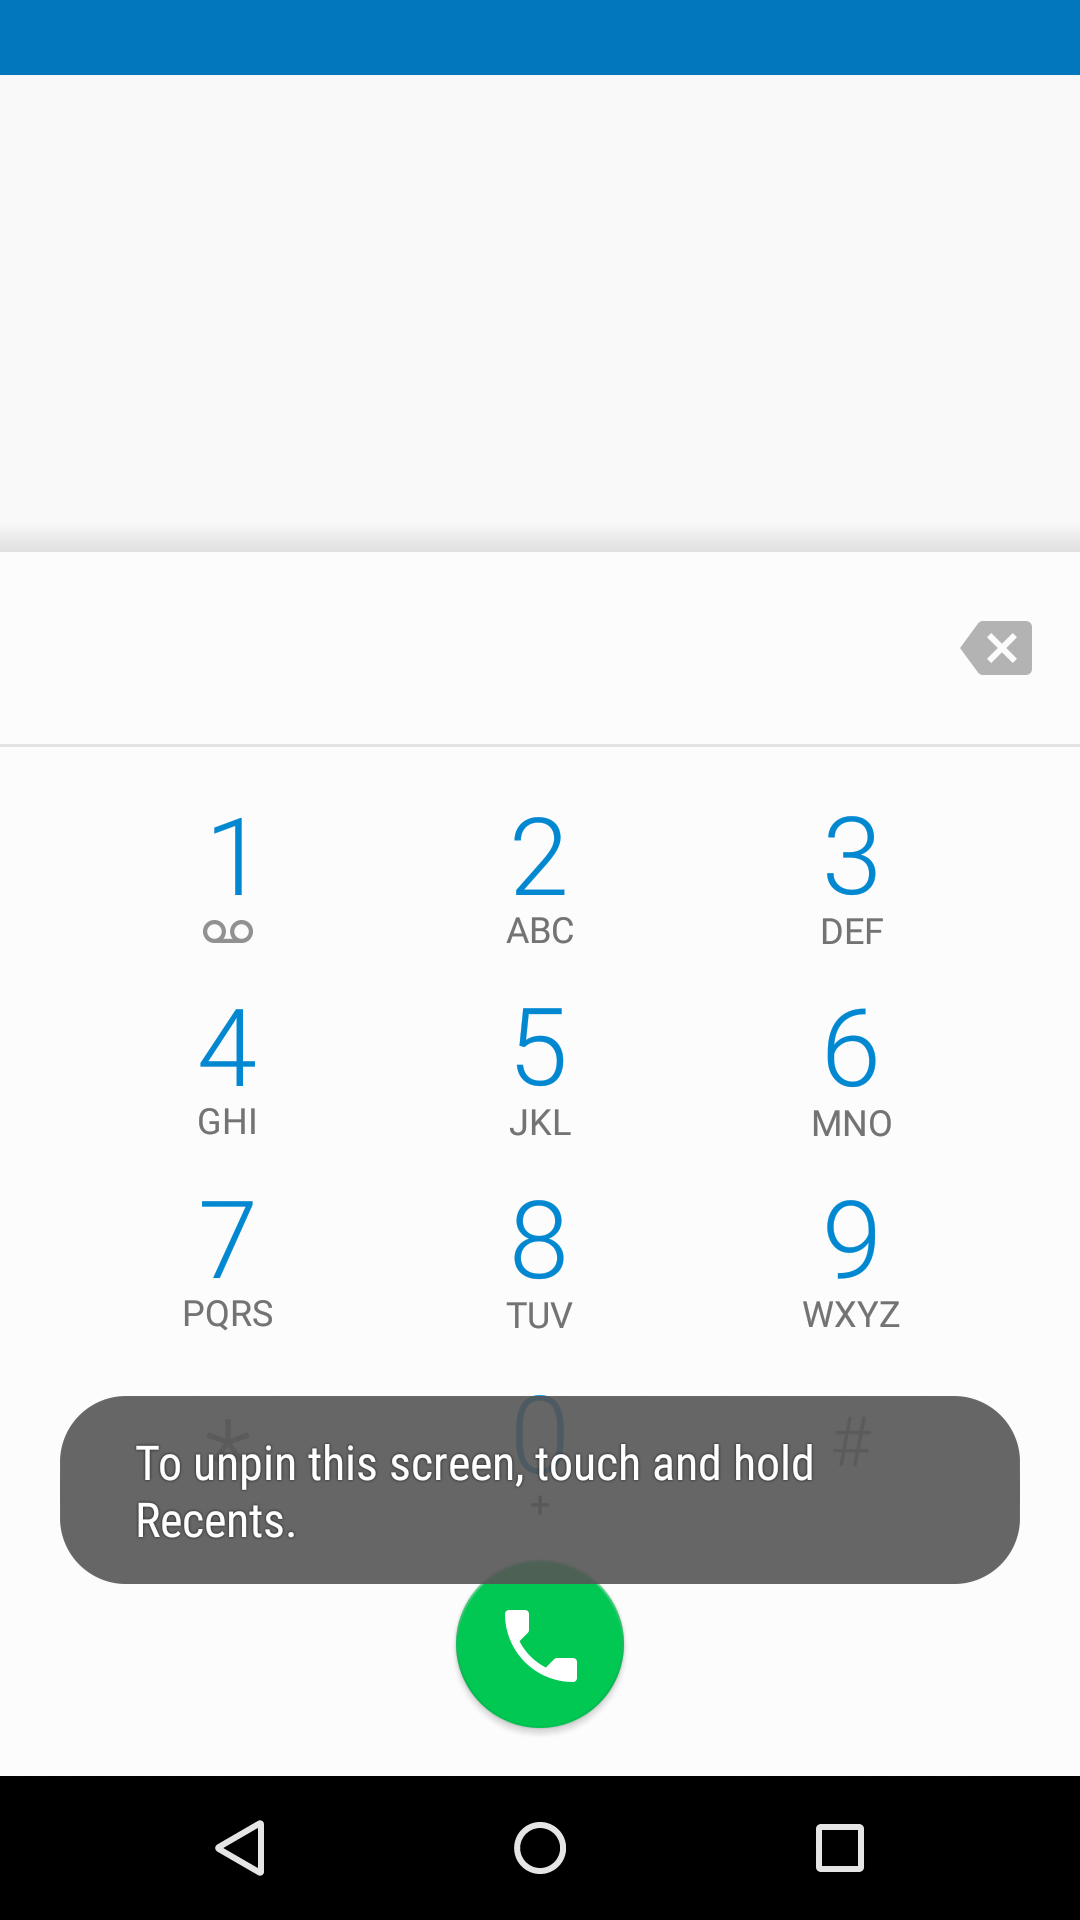
\includegraphics[width=0.8\linewidth]{figures/toast_example.png}
      \end{figure}
    \end{columns}
    \begin{exampleblock}{Example -- Creation and Display of a Toast}
      \begin{lstlisting}[language=Java]
CharSequence text = "Hello toast!";
Toast toast = Toast.makeText(getApplicationContext(), text, Toast.LENGTH_SHORT);
toast.show();
      \end{lstlisting}
    \end{exampleblock}
    \begin{itemize}\itemsep10pt
      \item The notification duration can be specified using
      \codeB{Toast.LENGTH\_SHORT} or \codeB{Toast.LENGTH\_LONG}.
      \item The \codeB{Toast} object offers some features that allow you to
      customize the notification.
    \end{itemize}
  \end{frame}

\section{Other types of Resources}

  \begin{frame}{Strings as Resources}
    \begin{itemize}\itemsep20pt
      \item On Android, it is best practice to never insert text messages (text
      strings) directly into the source code or as a value for the properties of
      GUI components. In this way it is possible to:
      \begin{itemize}
        \item Separate the contents
        \item Encourage the localization of application text in different
        languages
      \end{itemize} 
      \item By specifying the language setting, the resource file for the chosen
      text (if available) is loaded automatically
      \begin{itemize}
        \item In the source code, for each message, we will refer to the
        resource and not to the specific value. 
      \end{itemize}
    \end{itemize}
  \end{frame}

  \begin{frame}[fragile]{\texttt{strings.xml} File}
    \begin{itemize}
      \item It contains all the application resources of type \codeB{string}
      \item It must be placed in the \codeB{values} directory inside the
      \codeB{res} directory of the application project.
      \begin{itemize}
        \item Any other versions of the same file (with the same name) must be
        contained in directories at the same level of \codeA{values} with names such as
        \codeB{values-it}, \codeB{values-fr}, \dots
      \end{itemize}
    \end{itemize}

    \begin{exampleblock}{\texttt{strings.xml} file example}
      \begin{lstlisting}[language=XML]  		        
<?xml version="1.0" encoding="utf-8"?>
<resources>
  <string name="appName">MyFirstApp</string>
  <string name="btn01text">Click me!</string>
  <string name="settingsMenuLabel">Settings</string>
  <string name="myActivityTitle">MyActivity</string>
</resources>
      \end{lstlisting}
    \end{exampleblock}
  \end{frame}

  \begin{frame}[fragile]{Use of Textual Resources}
    \begin{itemize}
      \item From the other resources (e.g. layout), the resources of type
      \codeA{string} can be called by directly referring to the name of the
      resource with the prefix \codeA{@string}
    \end{itemize}
    \begin{exampleblock}{Use case}
      \begin{lstlisting}[language=XML]  		        
<Button android:id="@+id/mybutton"
  android:layout_width="wrap_content"
  android:layout_height="wrap_content"
  android:text="@string/btn01text"/>
      \end{lstlisting}
    \end{exampleblock}
    \begin{itemize}
      \item From the source code it's possible to use the \codeB{getString(int
      Id)} method provided by the \codeA{Context} class. 
    \end{itemize}
    \begin{exampleblock}{Use of textual resources in the source code}
      \begin{lstlisting}[language=Java]  		        
String s = getString(R.string.myActivityTitle);
      \end{lstlisting}
    \end{exampleblock}
  \end{frame}

\section{Shared Preferences}
  \begin{frame}{Shared Preferences}
    \begin{itemize}\itemsep10pt
      \item They represent the most naive mechanism for saving persistent
      information (data) in an Android application
      \begin{itemize}
        \item Persistent until the app is reinstalled on the system
      \end{itemize}
        \item They are data shared only by the components of the same
        application or accessible from the whole system, according to the chosen
        access level.
      \begin{itemize}
        \item \codeB{Context.MODE\_PRIVATE}: the data can only be read by the
        current application.
        \item \codeB{Context.MODE\_WORLD\_READABLE}: all applications will have
        Read-Only permissions on the data.
        \item \codeB{Context.MODE\_WORLD\_WRITEABLE}: all applications will have
        R/W permissions on the data.
      \end{itemize}
      \item For each application, the Shared Preferences must be associated with
      an identification name (a text string) 
    \end{itemize}
    \link{developer.android.com/reference/android/content/SharedPreferences.html}
  \end{frame}

\begin{frame}[fragile]{Shared Preferences -- Write Access}
  \begin{exampleblock}{Example -- Saving items in the Shared Preferences}
    \begin{lstlisting}[language=Java]  		        
final String PREFERENCES_ID = "my-app-preferences";
SharedPreferences preferences =
    getSharedPreferences(PREFERENCES_ID, Context.MODE_PRIVATE);

preferences.edit()
  .putString("USERNAME", "mario.rossi")
  .putString("PASSWORD","abc123")
  .putBoolean("LOGGED",true)
  .commit();
    \end{lstlisting}
  \end{exampleblock}
  \begin{itemize}
    \item The reference to the SPs can be obtained through the system API
    \codeB{getSharedPreferences(String id, int mode)}
    \begin{itemize}
      \item On this reference it is possible to add (save) data in the form key-value, by calling the SP Editor
      \item (1) invocation of the \codeB{edit()} method, (2) invocation of the
      various \codeA{putX(...)} methods, (3) invocation of the \codeB{commit()}
      method
    \end{itemize}
  \end{itemize}
\end{frame}

  \begin{frame}[fragile]{Shared Preferences -- Read Access}
    \begin{exampleblock}{Example -- Verification and Recovery of previously saved items}
      \begin{lstlisting}[language=Java]  		        
final String PREFERENCES_ID = "my-app-preferences";
        
SharedPreferences preferences =
   getSharedPreferences(PREFERENCES_ID, Context.MODE_PRIVATE);

String username = preferences.getString("USERNAME", "unavailable");
boolean logged = preferences.getBoolean("LOGGED", false);
      \end{lstlisting}
    \end{exampleblock}
    \begin{itemize}
      \item On the reference of the SPs, it is possible to invoke the
      \codeA{getX(...)} methods to obtain the value for the specified key.
      \item If the value is not available, the value of the second parameter of
      the \codeA{getX()} method will be returned as default.
    \end{itemize}
  \end{frame}

  \begin{frame}[fragile]{Shared Preferences -- Note}
    \begin{itemize}\itemsep10pt
      \item On the reference of the SPs (obtained through
      \codeA{getSharedPreferences()}) can be invoked the \codeB{getAll()}
      method. The latter returns a map (of type \codeB{Map<String,?>})
      containing all the elements of the SPs.
      \item You can register a listener who react to SP changes 
      \begin{itemize}
        \item The \codeB{registerOnSharedPreferenceChangeListener()} method
      \end{itemize}
    \end{itemize}
    \begin{exampleblock}{Example -- SP Callback}
      \begin{lstlisting}[language=Java]  		        
SharedPreferences.OnSharedPreferenceChangeListener spcl =
  new SharedPreferences.OnSharedPreferenceChangeListener() {
    @Override
    public void onSharedPreferenceChanged(
      SharedPreferences sp, String s
    ) { /* do something */ }
};
preferences.registerOnSharedPreferenceChangeListener(spcl);
      \end{lstlisting}
    \end{exampleblock}
  \end{frame}

\section*{References}

%-----------------------
%--- ONLINE RESURCES ---
%-----------------------

\begin{frame}{References - Online Resources}
\begin{thebibliography}{99}
\setbeamertemplate{bibliography item}[online]

\bibitem{adAPIguide} Android Developers - Guide
\newblock \link{https://developer.android.com/guide/}

\bibitem{adAPIreference} Android Developers - API Reference
\newblock \link{https://developer.android.com/reference/}

\bibitem{adTraining} Android Developers - Samples
\newblock \link{https://developer.android.com/samples/}

\bibitem{adTraining} Android Developers - Design \& Quality
\newblock \link{https://developer.android.com/design/}

\end{thebibliography}
\end{frame}

%-----------------------
%--- BOOKS -------------
%-----------------------

%\begin{frame}{Riferimenti - Libri}
%\begin{thebibliography}{99}
%\setbeamertemplate{bibliography item}[book]
%
%\bibitem{Mednieks11} Zigurd Mednieks, Laird Dornin, G. Blake Meike, Masumi Nakamura
%\newblock \emph{Programming Android}
%\newblock O'Reilly, 2011
%
%\bibitem{Haseman13} Chris Haseman, Kevin Grant
%\newblock \emph{Beginning Android Programming: Develop and Design}
%\newblock Peachpit Press, 2013
%
%\bibitem{Schwarz13} Ronan Schwarz, Phil Dutson, James Steele, Nelson To
%\newblock \emph{The Android Developer's Cookbook : Building Applications with the Android SDK}
%\newblock Addison-Wesley, 2013 
%
%\bibitem{Neil14} Theresa Neil
%\newblock \emph{Mobile Design Pattern Gallery: UI Patterns for Smartphone App}
%\newblock O'Relly, Second Edition, 2014
%\end{thebibliography}
%\end{frame}

\end{document}
